\documentclass[tikz,border=2pt]{standalone}
\usepackage{amsmath,amssymb}
\usepackage{tikz}
\usetikzlibrary{arrows.meta}

\begin{document}
% An infeasible LP: the constraints x_1 + x_2 <= 40 and x_1 + x_2 >= 60 (with x >= 0) have no
% common point, so the feasible region is empty.
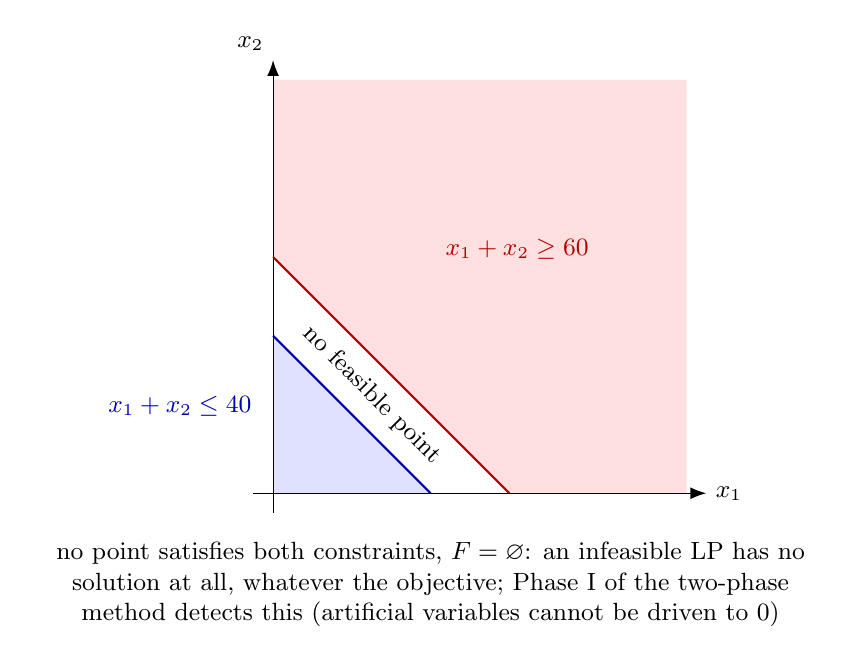
\begin{tikzpicture}[x=0.05cm, y=0.05cm, every node/.style={font=\small}, >={Latex[length=2mm]}]
	\fill[blue!12] (0,0) -- (40,0) -- (0,40) -- cycle;
	\fill[red!12] (60,0) -- (105,0) -- (105,105) -- (0,105) -- (0,60) -- cycle;
	\draw[->] (-5,0) -- (110,0) node[right] {$x_1$};
	\draw[->] (0,-5) -- (0,110) node[above left] {$x_2$};
	\draw[blue!70!black, thick] (40,0) -- (0,40);
	\draw[red!70!black, thick] (60,0) -- (0,60);
	\node[blue!70!black, font=\small, anchor=east] at (-3,22) {$x_1+x_2\le40$};
	\node[red!70!black, font=\small] at (62,62) {$x_1+x_2\ge60$};
	\node[font=\small, rotate=-45] at (25,25) {no feasible point};
	\node[anchor=north, align=flush center, text width=10cm] at (40,-10) {no point satisfies both constraints, $F=\varnothing$: an infeasible LP has no solution at all, whatever the objective; Phase I of the two-phase method detects this (artificial variables cannot be driven to $0$)};
\end{tikzpicture}
\end{document}
